\chapter{Planar Parameterization of Triangulated Surface Meshes}
\label{chap:surface_mesh_parameterization}
\ccChapterAuthor{Laurent Saboret, Pierre Alliez \and Bruno L\'evy}

\begin{ccPkgDescription}{Planar Parameterization of Triangulated Surface Meshes}
\ccPkgSummary{Parameterizing a surface amounts to finding a one-to-one mapping from
a suitable domain to the surface. In this package, we focus on
triangulated surfaces that are homeomorphic to a disk and on piecewise
linear mappings into a planar domain.  This \cgal\ package implements
some of the state-of-the-art surface mesh parameterization methods,
such as Least Squares Conformal Maps, Discrete Conformal Map, Discrete
Authalic Parameterization, Floater Mean Value Coordinates or Tutte
Barycentric Mapping.}

\ccPkgDependsOn{Solvers as \ccc{OpenNL} or \ccc{Taucs}.}
\ccPkgMaturity{Introduced in \cgal 3.2}

\end{ccPkgDescription}


\minitoc

\section{Introduction}

[TODO: replace next paragraphs by actual introduction]

We propose to elaborate upon a CGAL Package which implements some
of the state-of-the-art surface reconstruction methods. Priority will
be given to methods which take as input unorganized point sets and
which compute an implicit function, although we leave the room to
Delaunay-based techniques as all building blocks are available in
CGAL. A common implicit function is an approximate distance function
to the input points or to an estimate tangent plane, or an indicator
function.\\


The package will propose an interface to the CGAL Surface Mesh Generator~\cite{mariette06,oudot05},
and we leave the room to other surface contouring techniques such
as the Marching Cubes algorithm~\cite{37422} and its variants (a
user may prefer using his favorite contouring algorithm).\\


The input can be an unorganized point set, possibly with attributes
such as unoriented normals, oriented normals, confidence values. For
piecewise smooth reconstruction, it is also desirable to take not
only one attribute per point, but possibly several ones (for example,
two normals for a point on a sharp edge, or several normals for a
corner, or even a cone of normals). The input can also be a set of
arbitrary cross sections, be they defined by point sets localized
onto well-defined planes, or as polylines.\\


Since reconstruction methods often require to estimate and/or to orient
the normals of a point set, we plan to implement two components devoted
to this task. These components will make use of existing components
such as PCA or Jet fitting.\\


The output can be either an implicit function (ready for evaluation
by any contouring algorithm), or a surface mesh, compatible with the
BGL Graph concept and CGAL polyhedron when 2-manifold, or represented
as a polygon soup otherwise.


The intended audience of this package is researchers, developers or
students developing algorithms around surface reconstruction. We also
target end users and industrial applications.


\section{Basics}


\subsection{Poisson Reconstruction Overview}

Kazhdan, Bolitho and Hoppe introduced the Poisson Surface Reconstruction algorithm \cite{Kazhdan06}.
Given a set of 3D points with oriented normals (denoted oriented points in the sequel)
sampled on the boundary of a 3D solid, this method solves for an approximate indicator function of the inferred solid,
whose gradient best matches the input normals. The output scalar function, represented in an adaptive octree,
is then iso-contoured using an adaptive marching cubes.\\

\cgal\ implements a variant of this algorithm which solves for a piecewise linear function
on a 3D Delaunay triangulation instead of an adaptive octree.
The algorithm takes as input a set of 3D oriented points.
It builds a 3D Delaunay triangulation from these points and refines it by Delaunay refinement
so as to remove all badly shaped (non isotropic) tetrahedra and to tessellate a loose bounding box
of the input oriented points. The normal of each Steiner point added during refinement is set to zero.
It then solves for a scalar indicator function $f$ represented as a piecewise linear function over the refined triangulation.
More specifically, it solves for the Poisson equation  $\Delta f = div(\mathbf{n})$ at each vertex of the triangulation
using a sparse linear solver.
Eventually, the \cgal\ surface mesh generator extracts an isosurface with function value set by default
to be the median value of $f$ at all input points.

\subsection{Poisson Reconstruction API}

The class template declaration is:

template$<$  \\
class Gt,   \\
class \ccc{ReconstructionTriangulation_3}$>$   \\
class \ccc{Poisson_reconstruction_function};
\ccGlue
\ccCommentHeading{Parameters}
\begin{description}
\item \ccc{Gt}: Geometric traits class \item \ccc{ReconstructionTriangulation_3}: 3D Delaunay triangulation, model of \ccc{ReconstructionTriangulation_3} concept. \end{description}

The main constructor is:

\ccFunction{template<class InputIterator> Poisson_reconstruction_function(ReconstructionTriangulation_3& pdt, InputIterator first, InputIterator beyond);}
{
Creates a scalar function from a set of oriented points. Inserts the iterator range first...beyond into the triangulation pdt, refines it and solves for a piecewise linear scalar function which gradient best matches the input normals.
\ccPrecond the value type of InputIterator must be convertible to \ccc{Point_with_normal}.
\ccCommentHeading{Parameters}
\begin{description}
\item \ccc{pdt}: \ccc{ReconstructionTriangulation_3} base of the Poisson indicator function. \item \ccc{first}: First point to add. \item \ccc{beyond}: Past-the-end point to add. \end{description}
}

The main methods are:

\ccFunction{bool compute_implicit_function();}
{
The function \ccc{compute_implicit_function}() must be called after each insertion of oriented points. It computes the piecewise linear scalar function $f$ by:
\begin{itemize}
\item applying Delaunay refinement.
\item solving for $f$ at each vertex of the triangulation with a sparse linear solver.
\item shifting and orienting $f$ such that $f=0$ at all input points and $f<0$ inside the inferred surface.
\end{itemize}
Returns false on error.
}
\ccGlue
\ccFunction{FT value(const Point& p) const;}
{
Evaluates the implicit function at a given 3D query point.
}
\ccGlue
\ccFunction{Point get_inner_point() const;}
{
Returns a point located inside the inferred surface.
}
\ccFunction{Sphere bounding_sphere() const;}
{
Returns a sphere bounding the inferred surface.
}

See details in \\
\ccRefIdfierPage{CGAL::Poisson_reconstruction_function<GeomTraits, ReconstructionTriangulation_3>}


\subsection{Poisson Reconstruction Example}

\ccc{poisson_reconstruction_example.cpp} reads a point set, creates a Poisson implicit function and reconstructs a surface.

% I feel like we should further simplify it by providing
% just a list of oriented points.
\ccIncludeExampleCode{Point_set_processing_3/poisson_reconstruction_example.cpp}



\section{Surface Parameterization Methods
\label{sec:Surface-Parameterization-Methods}}

This \cgal\ package implements some of the state-of-the-art
surface parameterization methods, such as Least Squares Conformal Maps,
Discrete Conformal Map, Discrete Authalic
Parameterization, Floater Mean Value Coordinates or Tutte Barycentric
Mapping. These methods are provided as models of the
\ccc{ParameterizerTraits_3} concept.


\subsection{Fixed Border Surface Parameterizations}

Fixed Border Surface Parameterizations need a set of constraints: two
(u,v) coordinates for each vertex along the border.
Such border parameterizations are described in Section
\ref{sec:Border-Parameterizations-for-Fixed-Methods}.

\subsubsection{Tutte Barycentric Mapping}

\ccc{CGAL::Barycentric_mapping_parameterizer_3<ParameterizationMesh_3, BorderParameterizer_3, SparseLinearAlgebraTraits_d>}  \\

The Barycentric Mapping parameterization method has been introduced by
Tutte~\cite{t-hdg-63}. In parameter space, each vertex is
placed at the barycenter of its neighbors to achieve the so-called
convex combination condition. This algorithm amounts to solve one
sparse linear solver for each set of parameter coordinates, with a
\#vertices x \#vertices sparse and symmetric positive definite matrix
(if the border vertices are eliminated from the linear system).
A coefficient $(i, j)$ of the matrix is set to 1 for an edge linking
the vertex $v_i$ to the vertex $v_j$, to minus the degree of the
vertex $v_i$ for a diagonal element, and to 0 for any other matrix
entry. Although a bijective mapping is guaranteed when the border is convex,
this method does not minimize angles nor areas distortion.

% Tutte barycentric mapping
\begin{center}
    \label{Surface_mesh_parameterization-fig-uniform}
    % Image
    \begin{ccTexOnly}
      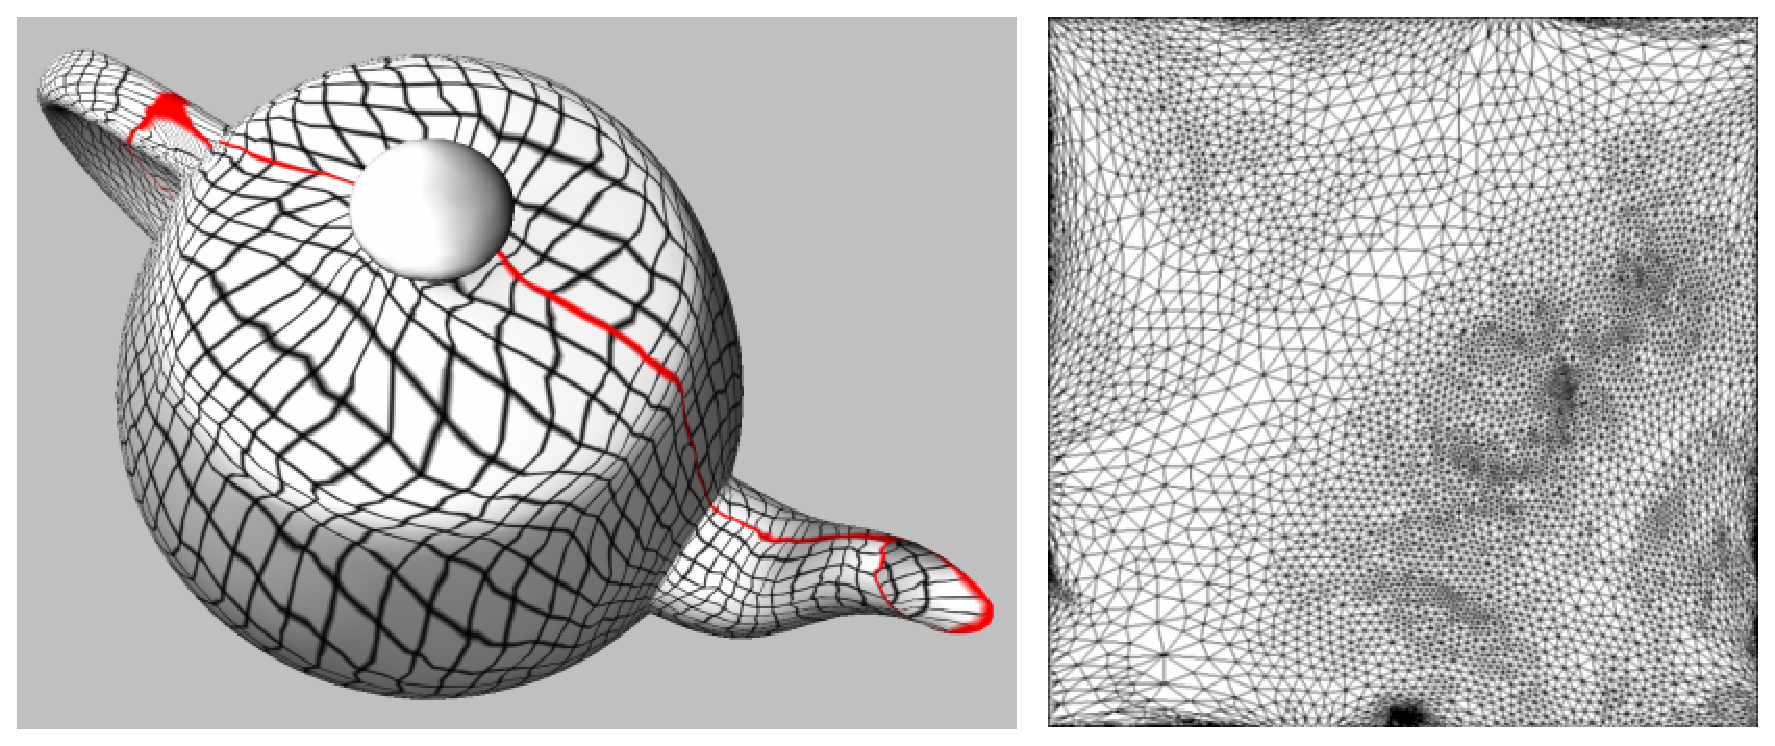
\includegraphics[width=1.0\textwidth]{Surface_mesh_parameterization/uniform}
    \end{ccTexOnly}
    \begin{ccHtmlOnly}
        <img style="max-width: 90%;" border=0 src="./uniform.png"><P>
    \end{ccHtmlOnly}
    % Title
    \begin{figure}[ht]
        \caption{Left: Tutte barycentric mapping parameterization (the red
                 line depicts the cut graph). Right: parameter space.}
    \end{figure}
\end{center}


\subsubsection{Discrete Conformal Map}

\ccc{CGAL::Discrete_conformal_map_parameterizer_3<ParameterizationMesh_3, BorderParameterizer_3, SparseLinearAlgebraTraits_d>}  \\

Discrete conformal map parameterization has been introduced by Eck et
al. to the graphics community~\cite{cgal:eddhls-maam-95}. It attempts to
lower angle deformation by minimizing a discrete version of the
Dirichlet energy as derived by Pinkall and
Polthier~\cite{cgal:pp-cdmsc-93}. A one-to-one mapping is guaranteed
only when the two following conditions are fulfilled: the barycentric mapping
condition (each vertex in parameter space is a convex combination if
its neighboring vertices), and the border is convex.
This method solves two \#vertices x \#vertices sparse linear
systems. The matrix (the same for both systems) is sparse and symmetric definite
positive (if the border vertices are eliminated from the linear system
and if the mesh contains no hole),
thus can be efficiently solved using dedicated linear solvers.

% Discrete conformal map
\begin{center}
    \label{Surface_mesh_parameterization-fig-conformal}
    % Image
    \begin{ccTexOnly}
        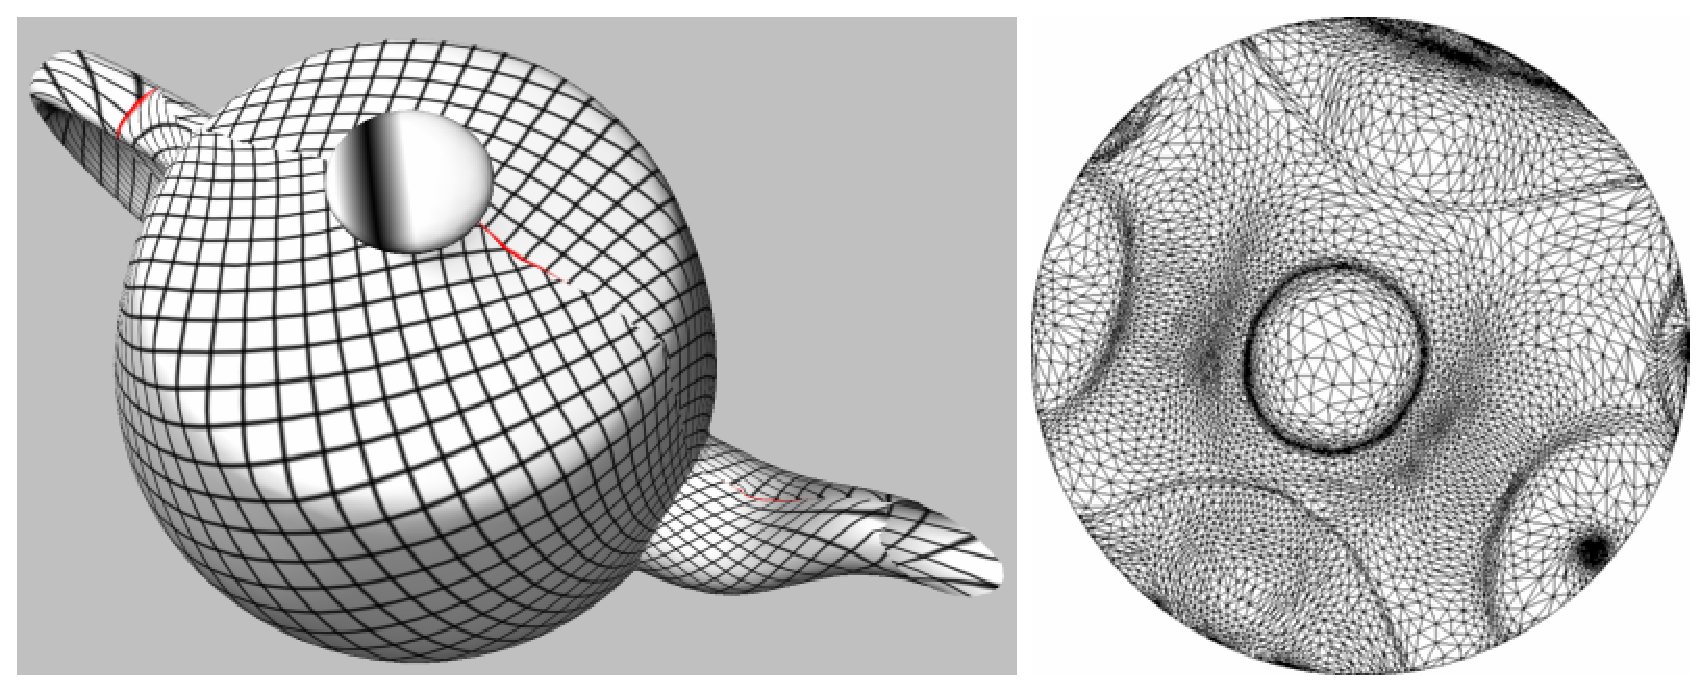
\includegraphics[width=1.0\textwidth]{Surface_mesh_parameterization/conformal}
    \end{ccTexOnly}
    \begin{ccHtmlOnly}
        <img style="max-width: 90%;" border=0 src="./conformal.png"><P>
    \end{ccHtmlOnly}
    % Title
    \begin{figure}[ht]
        \caption{Left: discrete conformal map. Right: parameter space.}
    \end{figure}
\end{center}

\subsubsection{Floater Mean Value Coordinates}

\ccc{CGAL::Mean_value_coordinates_parameterizer_3<ParameterizationMesh_3, BorderParameterizer_3, SparseLinearAlgebraTraits_d>}  \\

The mean value coordinates parameterization method has been introduced
by Floater~\cite{cgal:f-mvc-03}. Each vertex in parameter space is
optimized so as to be a convex combination of its neighboring
vertices. The barycentric coordinates are this time unconditionally
positive, by deriving an application of the mean theorem for harmonic
functions. This method is in essence an approximation of the discrete conformal
maps, with a guaranteed one-to-one mapping when the border is convex.
This method solves two \#vertices x \#vertices sparse linear systems. The matrix (the
same for both systems) is asymmetric.

% Floater mean value coordinates
\begin{center}
    \label{Surface_mesh_parameterization-fig-floater}
    % Image
    \begin{ccTexOnly}
      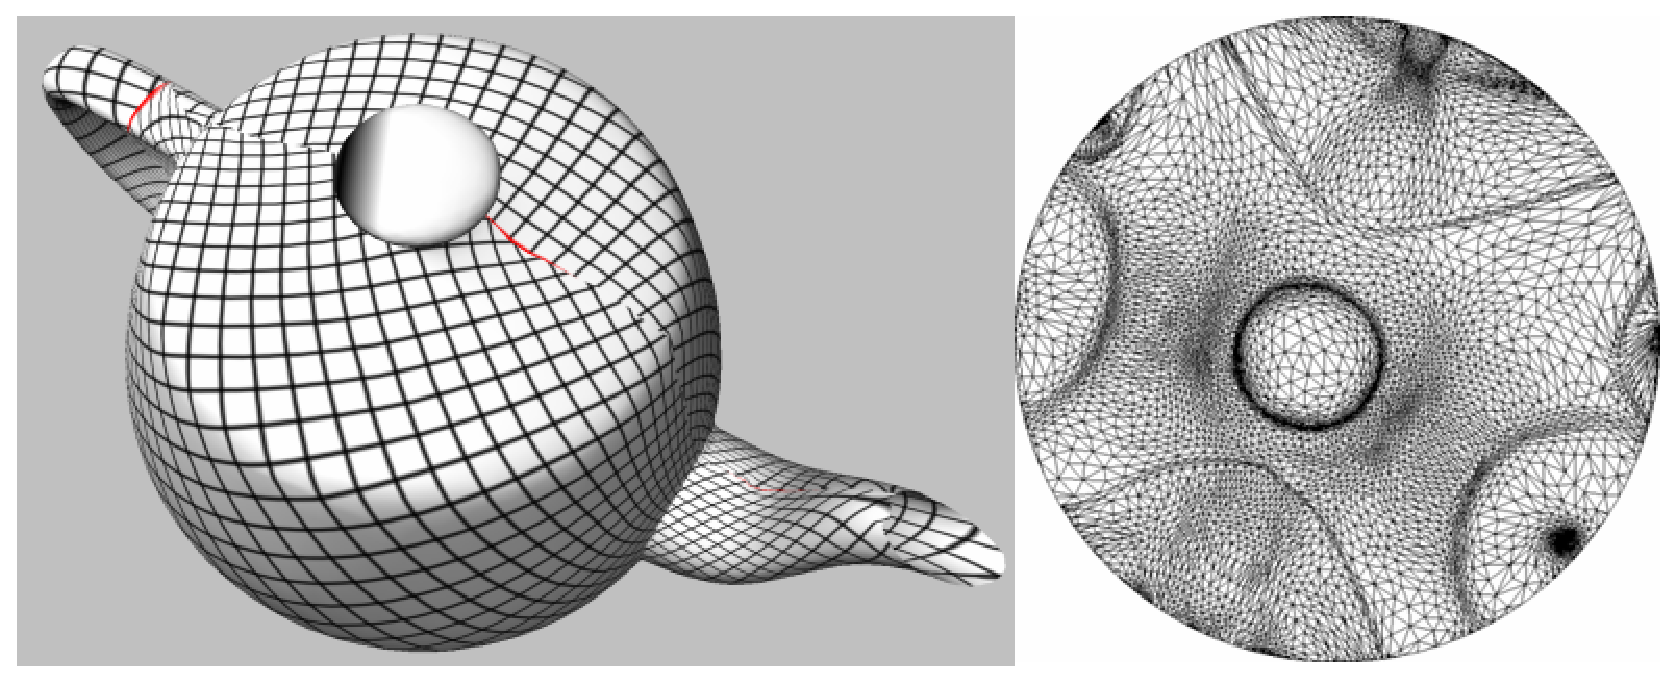
\includegraphics[width=1.0\textwidth]{Surface_mesh_parameterization/floater}
    \end{ccTexOnly}
    \begin{ccHtmlOnly}
        <img style="max-width: 90%;" border=0 src="./floater.png"><P>
    \end{ccHtmlOnly}
    % Title
    \begin{figure}[ht]
        \caption{Floater Mean Value Coordinates}
    \end{figure}
\end{center}

\subsubsection{Discrete Authalic parameterization}

\ccc{CGAL::Discrete_authalic_parameterizer_3<ParameterizationMesh_3, BorderParameterizer_3, SparseLinearAlgebraTraits_d>}  \\

The discrete authalic parameterization method has been introduced by
Desbrun et al.~\cite{cgal:dma-ipsm-02}. It corresponds to
a weak formulation of an area-preserving method, and in essence
locally minimizes the area distortion. A one-to-one mapping is
guaranteed only if the convex combination condition is fulfilled and
the border is convex. This method solves two
\#vertices x \#vertices sparse linear systems. The matrix (the same
for both systems) is asymmetric.

% Discrete authalic parameterization
\begin{center}
    \label{Surface_mesh_parameterization-fig-authalic}
    % Image
    \begin{ccTexOnly}
        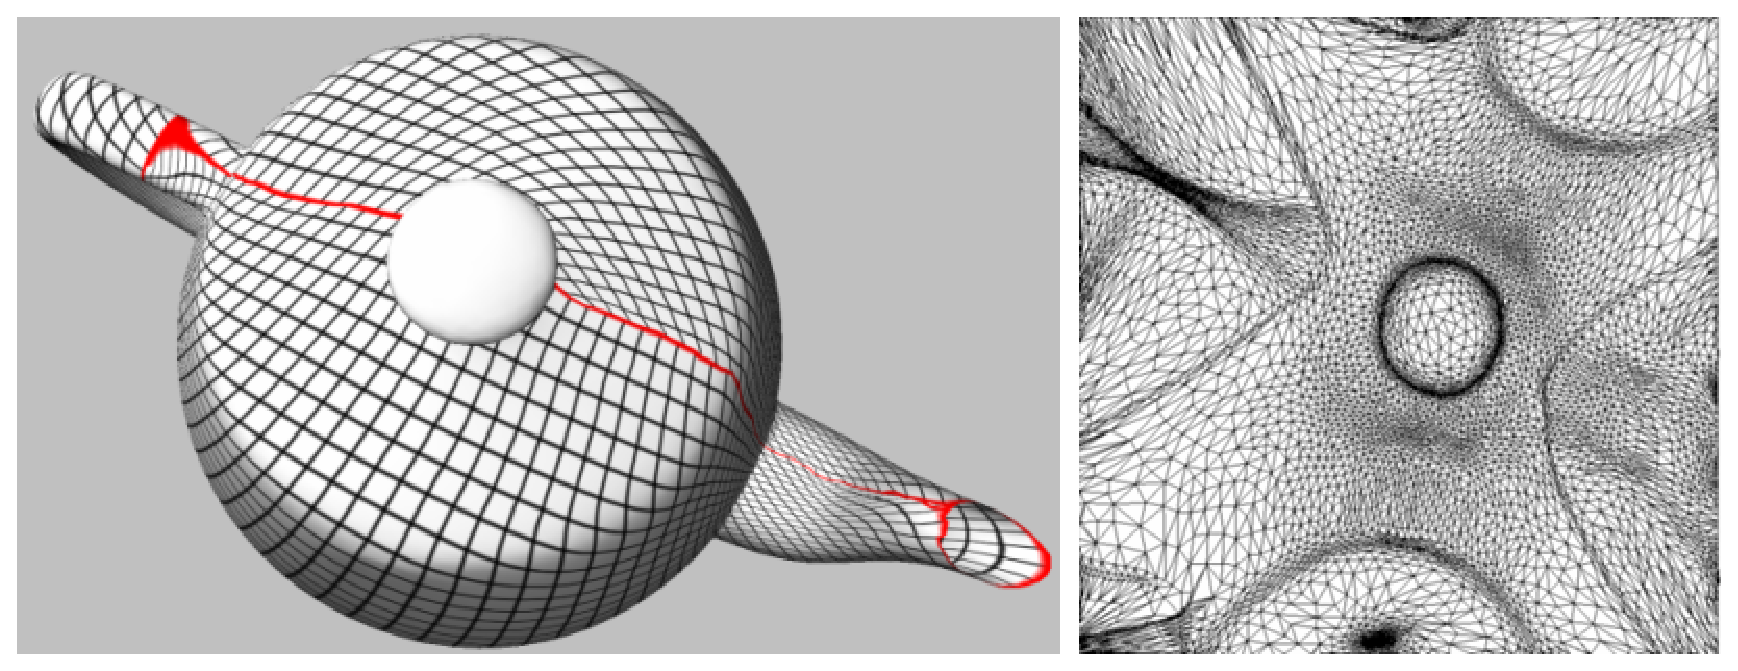
\includegraphics[width=1.0\textwidth]{Surface_mesh_parameterization/authalic}
    \end{ccTexOnly}
    \begin{ccHtmlOnly}
        <img style="max-width: 90%;" border=0 src="./authalic.png"><P>
    \end{ccHtmlOnly}
    % Title
    \begin{figure}[ht]
        \caption{Discrete Authalic Parameterization}
    \end{figure}
\end{center}

\subsubsection{Border Parameterizations for Fixed Methods
\label{sec:Border-Parameterizations-for-Fixed-Methods}}

Parameterization methods for
borders are used as traits classes modifying the behavior of
\ccc{ParameterizerTraits_3} models.
They are provided as models of the \ccc{BorderParameterizer_3} concept.
Border parameterizations for fixed border surface parameterizations
are a family of methods to define a set of constraints, namely two
$u,v$ coordinates for each vertex along the border.

\begin{itemize}

\item
    The user can select a border parameterization among
    two commonly used methods: uniform or arc-length parameterization.

    \emph{Usage:}

    Uniform border parameterization is more stable, although it gives
    poor visual results. The
    arc-length border parameterization is used by default.

\item
    One convex shape specified by one shape among two standard ones:
    a circle or a square.

    \emph{Usage:}

    The circular border parameterization is used by default as it
    corresponds to the simplest convex shape. The square border
    parameterization is commonly used for texture mapping.

\end{itemize}

\ccc{CGAL::Circular_border_arc_length_parameterizer_3<ParameterizationMesh_3>}  \\
\ccc{CGAL::Circular_border_uniform_parameterizer_3<ParameterizationMesh_3>}  \\
\ccc{CGAL::Square_border_arc_length_parameterizer_3<ParameterizationMesh_3>}  \\
\ccc{CGAL::Square_border_uniform_parameterizer_3<ParameterizationMesh_3>}  \\

% Julius Cesar mask circular vs square border
\begin{center}
    \label{Surface_mesh_parameterization-fig-circular_border}
    % Image
    \begin{ccTexOnly}
        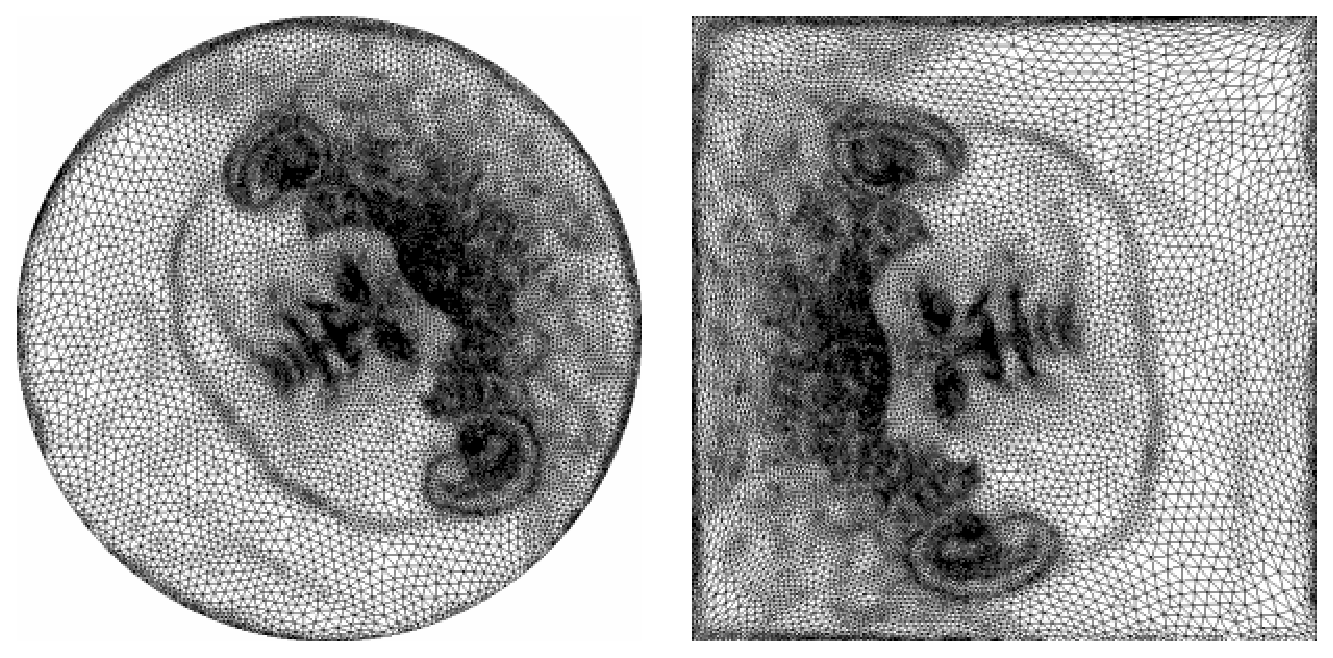
\includegraphics[width=1.0\textwidth]{Surface_mesh_parameterization/border}
    \end{ccTexOnly}
    \begin{ccHtmlOnly}
        <img style="max-width: 80%;" border=0 src="./border.png"><P>
    \end{ccHtmlOnly}
    % Title
    \begin{figure}[ht]
        \caption{Left: Julius Cesar mask parameterization with
                 Authalic/circular border. Right: Julius Cesar mask's
                 image with Floater/square border.}
    \end{figure}
\end{center}



\subsection{Free Border Surface Parameterizations}

\subsubsection{Least Squares Conformal Maps}

\ccc{CGAL::LSCM_parameterizer_3<ParameterizationMesh_3, BorderParameterizer_3, SparseLinearAlgebraTraits_d>}  \\

The Least Squares Conformal Maps (LSCM) parameterization method has
been introduced by L\'evy et al.~\cite{cgal:lprm-lscm-02}.
It corresponds to a conformal method with a free border (at least two
vertices have to be constrained to obtain a unique solution), which
allows further lowering of the angle distortion. A one-to-one mapping
is not guaranteed by this method. It solves a (2 $\times$
\#triangles) $\times$ \#vertices sparse linear system in the least squares sense,
which implies solving a symmetric matrix.

% LSCM
\begin{center}
    \label{Surface_mesh_parameterization-fig-LSCM}
    % Image
    \begin{ccTexOnly}
        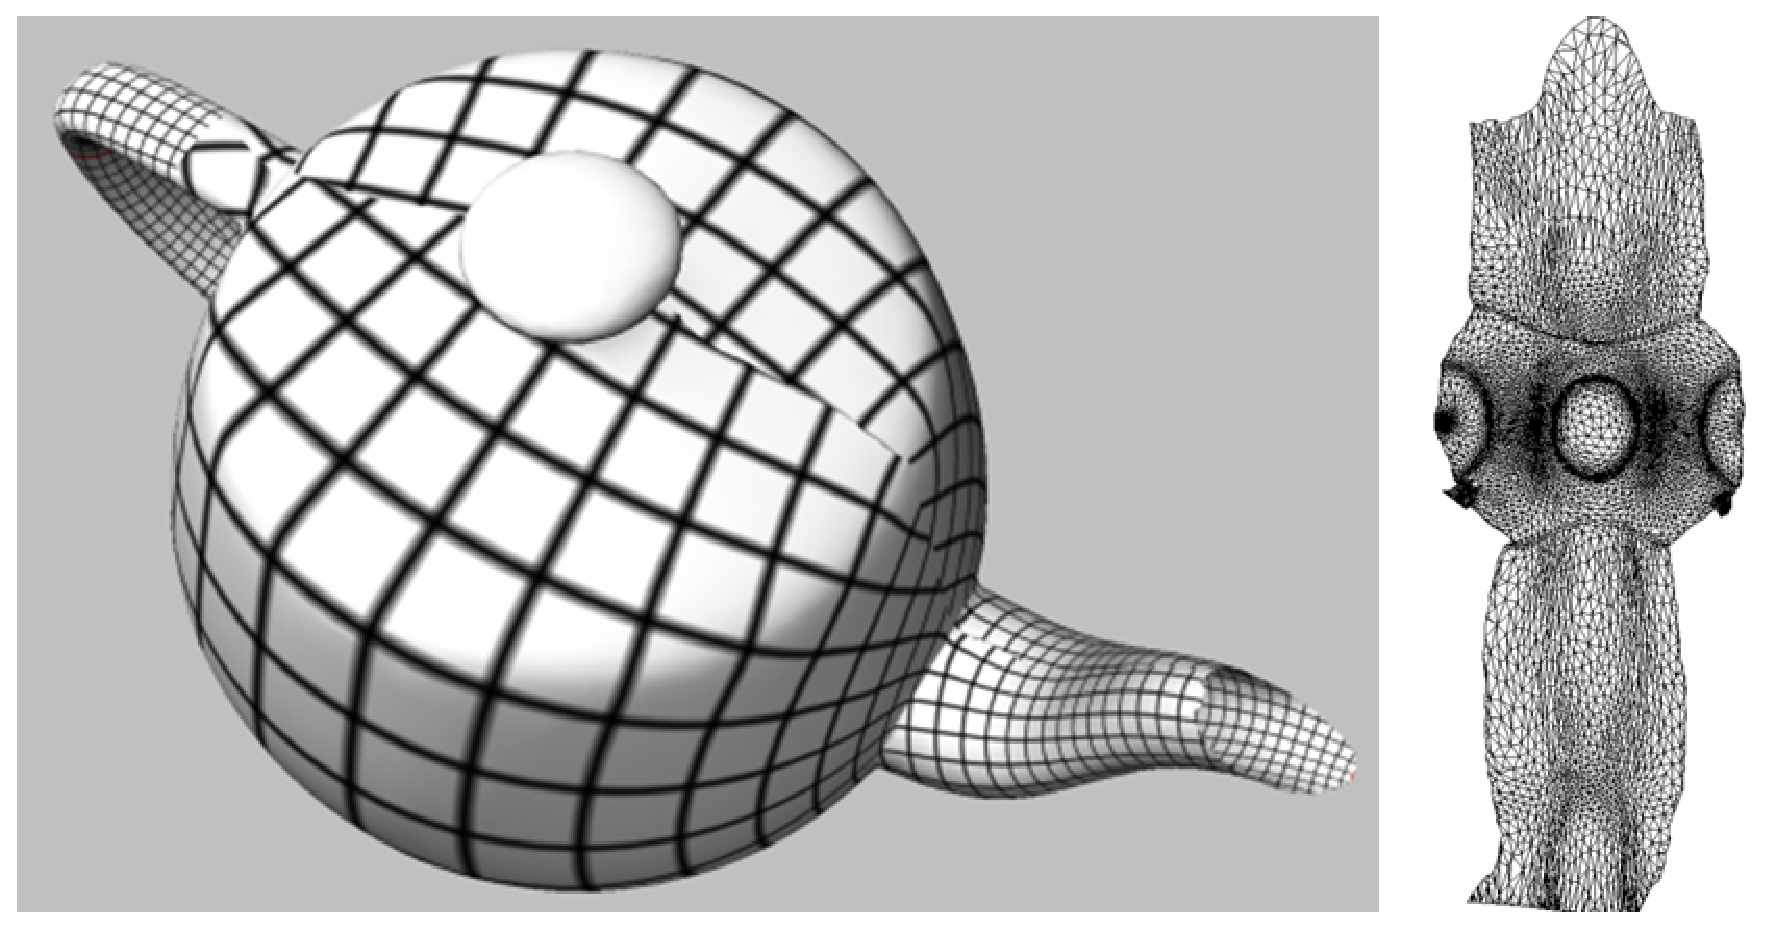
\includegraphics[width=1.0\textwidth]{Surface_mesh_parameterization/LSCM}
    \end{ccTexOnly}
    \begin{ccHtmlOnly}
        <img style="max-width: 90%;" border=0 src="./LSCM.png"><P>
    \end{ccHtmlOnly}
    % Title
    \begin{figure}[ht]
        \caption{Least squares conformal maps.}
    \end{figure}
\end{center}


\subsubsection{Border Parameterizations for Free Methods
\label{sec:Border-Parameterizations-for-Free-Methods}}

Parameterization methods for
borders are used as traits classes modifying the behavior of
\ccc{ParameterizerTraits_3} models. They are provided as models of the \ccc{BorderParameterizer_3} concept.
The border parameterizations associated to free border surface
parameterization methods define only two constraints: the pinned vertices.

\begin{itemize}

\item
    \ccc{CGAL::Two_vertices_parameterizer_3<ParameterizationMesh_3>}  \\

    \emph{Usage:}

    \ccc{CGAL::Two_vertices_parameterizer_3<ParameterizationMesh_3>} is the default
    free border parameterization, and is the only one available
    in the current version of this package.

\end{itemize}


\subsection{Discrete Authalic Parameterization Example}

\ccc{Authalic_parameterization.cpp} computes a Discrete Authalic parameterization
over a \ccc{CGAL::Polyhedron_3<Traits>} mesh. Specifying a specific surface parameterization
instead of the default one means using the second parameter of \ccc{CGAL::parameterize()}. The
differences with the first example \ccc{Simple_parameterization.cpp} are:

\begin{ccExampleCode}

#include <CGAL/Discrete_authalic_parameterizer_3.h>

...

//***************************************
// Discrete Authalic Parameterization
//***************************************

typedef CGAL::Discrete_authalic_parameterizer_3<Parameterization_polyhedron_adaptor>
                                                    Parameterizer;

Parameterizer::Error_code err = CGAL::parameterize(mesh_adaptor, Parameterizer());

...

\end{ccExampleCode}


\subsection{Square Border Arc Length Parameterization Example}

\ccc{Square_border_parameterization.cpp} computes a Floater mean value coordinates
parameterization with a square border arc length parameterization.
Specifying a specific border parameterization
instead of the default one means using the second parameter of
\ccc{CGAL::Mean_value_coordinates_parameterizer_3<ParameterizationMesh_3, BorderParameterizer_3, SparseLinearAlgebraTraits_d>}.
The differences with the first example \ccc{Simple_parameterization.cpp} are:

\begin{ccExampleCode}

#include <CGAL/Square_border_parameterizer_3.h>

...

//***************************************
// Floater Mean Value Coordinates parameterization
// with square border
//***************************************

// Square border parameterizer
typedef CGAL::Square_border_arc_length_parameterizer_3<Parameterization_polyhedron_adaptor>
                                                        Border_parameterizer;

// Floater Mean Value Coordinates parameterizer with square border
typedef CGAL::Mean_value_coordinates_parameterizer_3<Parameterization_polyhedron_adaptor,
                                                        Border_parameterizer>
                                                    Parameterizer;

Parameterizer::Error_code err = CGAL::parameterize(mesh_adaptor, Parameterizer());

...

\end{ccExampleCode}


\section{Sparse Linear Algebra}

\subsection{Solvers List and Concept}

We provide an interface to several state-of-the-art
sparse linear solvers, as models of the SparseLinearAlgebraTraits\_d concept:

\begin{itemize}

\item OpenNL (Bruno L{\'e}vy) is shipped with \cgal. This is the default solver.

OpenNL::DefaultLinearSolverTraits  \\
OpenNL::SymmetricLinearSolverTraits  \\

\item TAUCS is a reference direct solver for sparse symmetric matrices.

\ccRefIdfierPage{CGAL::Taucs_solver_traits}  \\
\ccRefIdfierPage{CGAL::Taucs_symmetric_solver_traits}  \\

\item SuperLU is a reference direct solver for sparse unsymmetric matrices.

(traits class not yet implemented)

\end{itemize}


\subsection{TAUCS Solver Example}

The code above uses the default sparse linear solver: OpenNL.

The code below applies the default parameterization method
(Floater's mean value coordinates with a circular border),
but specifically instantiates TAUCS solver:

\begin{ccExampleCode}

// CGAL kernel
typedef CGAL::Cartesian<double>                         Kernel;

// Mesh true type and parameterization adaptors
typedef CGAL::Polyhedron_3<Kernel>                      Polyhedron;
typedef CGAL::Mesh_adaptor_polyhedron_3<Polyhedron>     Mesh_adaptor_polyhedron;

// Circular border parametizer (the default)
typedef CGAL::Circular_border_arc_length_parametizer_3<Mesh_adaptor_polyhedron>
                                                        Border_parametizer;
// TAUCS solver
typedef CGAL::Taucs_solver_traits<double>               Solver;

// Floater's mean value coordinates parametizer (circular border)
// with TAUCS solver
typedef CGAL::Mean_value_coordinates_parametizer_3<Mesh_adaptor_polyhedron,
                                                   Border_parametizer,
                                                   Solver>
                                                        Parametizer;

int main(int argc,char * argv[])
{
    Polyhedron mesh;
    ...

    // The parameterization package needs an adaptor to handle Polyhedron_3 meshes
    Mesh_adaptor_polyhedron mesh_adaptor(&mesh);

    // Floater's mean value coordinates parametizer (circular border)
    // with TAUCS solver
    Parametizer::Error_code err = CGAL::parameterize(&mesh_adaptor, Parametizer());
    ...
}

\end{ccExampleCode}

See the complete code in Polyhedron\_parameterization4.C example.


\section{Cutting a Mesh}

\subsection{Computing a Cut}

All surface parameterization methods proposed in this package only
deal with topological discs.  The input mesh can be of any genus and
have any number of connected components, but if it is not a topological
disc, it has to come with a description of a border (an oriented list of
vertices) which is the border of a topological disc.  If no border  is
given as input, we assume that the surface border is the longest border already
in the input mesh (the other borders will be considered as holes).

% pierre: big contradiction here - it can be something else than a
% disk then!

This package does not provide any algorithm to transform a closed mesh
of arbitrary genus into a topological disk, the user being responsible
for computing such a cut. Nevertheless we provide in
\ccc{polyhedron_ex_parameterization.C} a simple cutting algorithm for
the sake of completeness.


\subsection{Applying a Cut}

Parameterization methods in this package only support triangulated
surfaces that are homeomorphic to a disk (models of
\ccc{ParameterizationMesh_3}). This software design simplifies the
implementation of all new parameterization methods based on linear
solvers.

\ccc{Parameterization_mesh_patch_3} class is responsible for virtually
{\em cutting} a patch to a \ccc{ParameterizationPatchableMesh_3} mesh,
to make it similar ffromt he interface point of view to a topological
disk with a \ccc{ParameterizationMesh_3} interface.

\ccc{ParameterizationPatchableMesh_3} inherits from concept \ccc{ParameterizationMesh_3}, thus is a concept for a 3D surface mesh.
\ccc{ParameterizationPatchableMesh_3} adds the ability to support patches and virtual seams. Patches are a subset of a 3D mesh. Virtual seams are the ability to behave exactly as if the surface was {\em cut} following a certain path.

The \ccc{ParameterizationMesh_3} interfaces with both the 2D
Triangulation Data Structure enriched with 3D points (not yet
implemented) and the Polyhedron are also models of
\ccc{ParameterizationPatchableMesh_3}:

\ccc{CGAL::Parameterization_polyhedron_adaptor_3}  \\


\subsection{Cutting a Mesh Example}

The code below virtually {\em cuts} a \ccc{Polyhedron_3} mesh to make
it a topological disk, then applies the default parameterization:

\begin{ccExampleCode}

// CGAL kernel
typedef CGAL::Cartesian<double>                             Kernel;

// Mesh true type and parameterization adaptors
typedef CGAL::Polyhedron_3<Kernel>                          Polyhedron;
typedef CGAL::Parameterization_polyhedron_adaptor_3<Polyhedron>
                                                            Parameterization_polyhedron_adaptor;
typedef CGAL::Parameterization_mesh_patch_3<Parameterization_polyhedron_adaptor>
                                                            Mesh_patch_polyhedron;

// Parameterizers base class for this kind of mesh
typedef CGAL::Parameterizer_traits_3<Mesh_patch_polyhedron> Parameterizer;

// Type describing a border or seam as a vertex list
typedef std::list<Parameterization_polyhedron_adaptor::Vertex_handle>
                                                            Seam;

// If the mesh is a topological disk, extract its longest border,
// else compute a very simple cut to make it homeomorphic to a disk.
// Return the border/seam (empty on error)
static Seam cut_mesh(Parameterization_polyhedron_adaptor* mesh_adaptor)
{
    // To be implemented by package user
    ...
}

int main(int argc,char * argv[])
{
    Polyhedron mesh;
    ...

    // The Surface_mesh_parameterization package needs an adaptor to handle Polyhedron_3 meshes
    Parameterization_polyhedron_adaptor mesh_adaptor(&mesh);

    // The parameterization methods support only meshes that
    // are topological disks => we need to compute a "cutting" of the mesh
    // that makes it it homeomorphic to a disk
    Seam seam = cut_mesh(&mesh_adaptor);

    // Create adaptor that virtually "cuts" the mesh following the 'seam' path
    Mesh_patch_polyhedron   mesh_patch(&mesh_adaptor,
                                       seam.begin(),
                                       seam.end());

    // Floater Mean Value Coordinates parameterization
    Parameterizer::Error_code err = CGAL::parameterize(&mesh_patch);
    ...
}

\end{ccExampleCode}

See the complete example in \ccc{Mesh_cutting_parameterization.C}
example.



\section{Output}

Parameterization methods compute $(u,v)$ fields for each vertex
of the input mesh, with the seam vertices being virtually duplicated (thanks
to \ccc{Parameterization_mesh_patch_3<ParameterizationPatchableMesh_3>}).

To support this duplication,
\ccc{Parameterization_polyhedron_adaptor_3<Polyhedron_3_>} stores
the result in the $(u,v)$ fields of the input mesh halfedges.
A $(u,v)$ pair is provided for
each inner vertex (i.e. its halfedges share the same $(u,v)$ pair),
while a $(u,v)$ pair is provided for each seam halfedge.
The user has to iterate over the mesh halfedges to get the result.

Note: $(u,v)$ fields do not exist in CGAL \ccc{Polyhedron_3},
thus the output traversal is specific to the way the (u,v) fields are implemented by the adaptor.

\subsection{EPS Output Example}

\ccc{Complete_parameterization_example.C} is a complete parameterization
example that outputs the result as an EPS image.
It gets the $(u,v)$ fields computed by a
parameterization method over a \ccc{Polyhedron_3} mesh with a
\ccc{Parameterization_polyhedron_adaptor_3<Polyhedron_3_>} adaptor:

\ccIncludeExampleCode{Surface_mesh_parameterization/Complete_parameterization_example.C}


\section{Complexity and Guarantees}


\subsection{Parameterization Methods and Guarantees}

\begin{itemize}

\item Fixed boundaries

    \begin{itemize}

    \item One-to-one mapping

        Tutte's theorem guarantees a one-to-one mapping provided that the weights are all positive
        and the border convex.
        It is the case for Tutte barycentric mapping and Floater mean value coordinates.
        It is not always the case for discrete conformal map (cotangents) and
        discrete authalic parameterization.

    \item Non-singularity of the matrix

        Geshorgin's theorem guarantees the convergence of the solver if the matrix is diagonal dominant.
        This is the case with positive weights (Tutte barycentric mapping and Floater mean value coordinates).

    \end{itemize}

\item Free boundaries

    \begin{itemize}

    \item One-to-one mapping

        No guarantee is provided by LSCM (both global overlaps and triangle flips can
        occur).

    \item Non-singularity of the matrix

        For LSCM, the matrix of the system is the Gram matrix of a matrix with maximal rank,
        and is therefore non-singular (Gram theorem).

    \end{itemize}

\end{itemize}


\subsection{Precision}

Two algorithms of this package construct the sparse linear system(s)
using trigonometric functions, and are this incompatible with exact arithmetic:

\begin{itemize}

\item Floater mean value coordinates

\item Circular border parameterization

\end{itemize}

On the other hand, linear solvers commonly use double precision floating point
numbers. \\
OpenNL's BICGSTAB solver (accessible through the
\ccc{OpenNL::DefaultLinearSolverTraits<COEFFTYPE, MATRIX, VECTOR, SOLVER>} interface)
is the only solver supported by this package which 
computes exact results, when used with an exact arithmetic. This package is
intended to be used mainly with a \cgal\ Cartesian kernel with doubles.


\subsubsection{OpenNL's BICGSTAB Solver with an Exact Arithmetic}

The BICGSTAB conjugate gradient is in disguise a direct solver.
In a nutshell, it computes a vector basis
orthogonal with respect to the matrix, and the coordinates of the solution in this vector basis.
Each iteration computes one component of the basis and one coordinate, therefore the algorithm
converges to the solution in $n$ iterations, where $n$ is the dimension of the matrix. More precisely, it is shown to converge in $k$ iteration, where $k$ is the number of distinct eigenvalues of the matrix. 

% For a perfectly conditioned matrix, it converges in a single iteration.

\subsubsection{Solvers with a Floating Point Arithmetic}

\emph{OpenNL's BICGSTAB example:}

When inexact numerical types are used (e.g. doubles), accumulated errors slow down convergence
(in practice, it requires approximately $5k$ iterations to converge).
The required number of iterations depends on the eigenvalues of the matrix, and these eigenvalues depend
on the shape of the triangles. The optimum is when the triangles are equilateral (then the solver converges
in less than 10 iterations). The worst case is obtained when the mesh has a large number of skinny triangles (near-singular Jacobian matrix of the triangle). In this case, the spectrum of the matrix
is wide (many different eigenvalues), and the solver requires nearly $5n$ iterations to converge.


\subsection{Algorithmic Complexity}

In this package, we focus on piecewise linear mappings onto a planar
domain. All surface parameterization methods are based on solving one (or two)
sparse linear system(s).
The algorithmic complexity is dominated by the resolution of the sparse linear system(s).

\emph{OpenNL's BICGSTAB example:}

At each iteration, the operation of highest complexity is the product between the sparse-matrix and a vector.
The sparse matrix has a fixed number of non-zero coefficients per row,
therefore the matrix / vector product has $O(n)$ complexity.
Since convergence is reached after $k$ iterations, the complexity is $O(k.n)$
(where $k$ is the number of distinct eigenvalues of the matrix).
Therefore, best case complexity is $O(n)$ (equilateral triangles),
and worst case complexity is $O(n^2)$ (skinny triangles).


\section{Software Design}

\subsection{Global Function parameterize()}

This package's entry point is:

\begin{ccExampleCode}
// Compute a one-to-one mapping from a 3D triangle surface 'mesh' to a
// 2D circle, using Floater Mean Value Coordinates algorithm.
// A one-to-one mapping is guaranteed.
template <class ParameterizationMesh_3>
typename Parameterizer_traits_3<ParameterizationMesh_3>::Error_code
parameterize(ParameterizationMesh_3& mesh)  // 3D mesh, model of ParameterizationMesh_3 concept
{
    Mean_value_coordinates_parameterizer_3<ParameterizationMesh_3> parameterizer;
    return parameterizer.parameterize(mesh);
}

// Compute a one-to-one mapping from a 3D triangle surface 'mesh' to a
// simple 2D domain.
// One-to-one mapping may be guaranteed or not,
// depending on the chosen ParametizerTraits_3 algorithm.
template <class ParameterizationMesh_3, class ParameterizerTraits_3>
typename Parameterizer_traits_3<ParameterizationMesh_3>::Error_code
parameterize(ParameterizationMesh_3& mesh,          // 3D mesh, model of ParameterizationMesh_3
             ParameterizerTraits_3 parameterizer)   // Parameterization method for 'mesh'
{
    return parameterizer.parameterize(mesh);
}
\end{ccExampleCode}

You may notice that these global functions simply call the
parameterize() method of a \ccc{ParameterizerTraits_3} object.
The purpose of these global functions is:
\begin{itemize}
\item to be consistent with other \cgal\ algorithms that are also provided as
      global functions, e.g. \ccc{CGAL::convex_hull_2()},
\item to provide a default parameterization method (Floater Mean Value Coordinates),
      which wouldn't be possible with a direct call to an object's method.
\end{itemize}

You may also wonder why there is not just one \ccc{CGAL::parameterize()} function
with a default \ccc{ParameterizerTraits_3} argument equal to
\ccc{CGAL::Mean_value_coordinates_parameterizer_3<ParameterizationMesh_3>}.
The reason is simply that this is not allowed by the C++ standard (see
\cite{cgal:ansi-is14882-98}, paragraph 14.1/9).


\subsection{No Common Parameterization Algorithm}

\ccc{ParameterizerTraits_3} models modify the behavior of the global function
\ccc{CGAL::parameterize()} - hence the {\em Traits} in the name.
On the other hand, \ccc{ParameterizerTraits_3} models do not modify the behavior
of a common parameterization algorithm - as you might expect.

In this package, we focus on triangulated surfaces that are homeomorphic to a
disk and on piecewise linear mappings onto planar domains.
A consequence is that the skeleton of all parameterization methods of this
package is the same:
\begin{itemize}
\item Allocate a sparse linear system $A.X = B$
\item Parameterize the mesh border and initialize $B$
\item Parameterize the inner points of the mesh and set $A$ coefficients
\item Solve the system
\end{itemize}

It is tempting to make the parameterization method a traits class that
modifies the behavior of a common parameterization algorithm.
On the other hand, there are several differences among methods:
\begin{itemize}
\item Fixed border methods need to parameterize all border vertices,
      while free border methods parameterize only two vertices.
\item Some methods create symmetric definite positive systems,
      which may be solved more efficiently than general systems.
\item Most parameterization methods use two \#vertices x \#vertices systems,
      where Least Squares Conformal Maps uses one (2 * \#triangles) x \#vertices system.
\item Most parameterization methods invert the $A$ matrix,
      when Least Squares Conformal Maps solves the system in the least squares sense.
\end{itemize}

Therefore, the software design chosen is:
\begin{itemize}
\item Each \ccc{ParameterizerTraits_3} model implements its own version
      of the parameterization algorithm as a parameterize() method.
\item Each \ccc{ParameterizerTraits_3} model has template arguments
      defining the border parameterization and sparse linear solver to use,
      with default values adapted to the method.
\item Code factorization is achieved using a class hierarchy and (few) virtual methods.
\end{itemize}

% Insert image parameterizer_class_diagram.png/eps with title
% "A parameterizer UML class diagram (main types and methods only)" and scale = 1:1
\begin{center}
    \label{Surface_mesh_parameterization-fig-parameterizer_class_diagram}
    % Image
    \begin{ccTexOnly}
        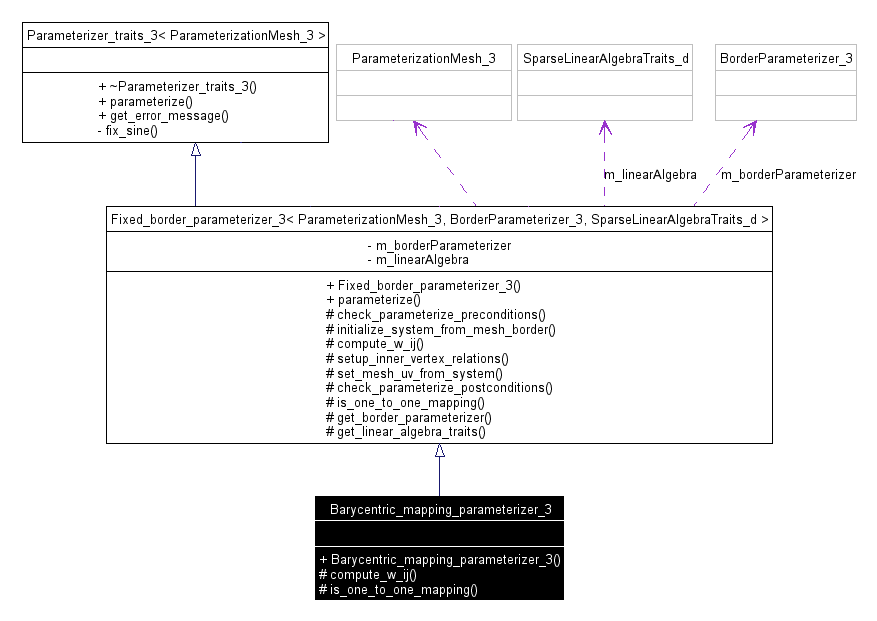
\includegraphics[width=1.0\textwidth]{Surface_mesh_parameterization/parameterizer_class_diagram}
    \end{ccTexOnly}
    \begin{ccHtmlOnly}
        <img style="max-width: 100%;" border=0 src="./parameterizer_class_diagram.png"><P>
    \end{ccHtmlOnly}
    % Title
    \begin{figure}[h]
        \caption{A parameterizer UML class diagram (main types and methods only)}
    \end{figure}
\end{center}

% Insert image parameterizers_class_hierarchy.png/eps with
% title "Surface parameterizer classes hierarchy" and scale = 1:1
\begin{center}
    \label{Surface_mesh_parameterization-fig-parameterizers_class_hierarchy}
    % Image
    \begin{ccTexOnly}
        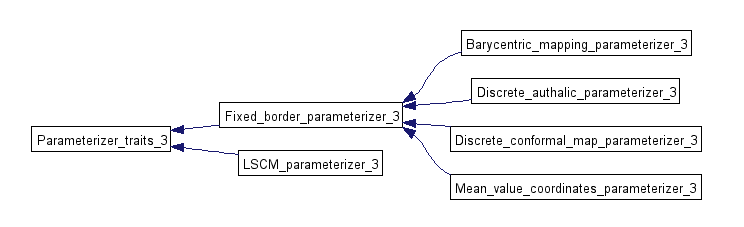
\includegraphics[width=1.0\textwidth]{Surface_mesh_parameterization/parameterizers_class_hierarchy}
    \end{ccTexOnly}
    \begin{ccHtmlOnly}
        <img style="max-width: 100%;" border=0 src="./parameterizers_class_hierarchy.png"><P>
    \end{ccHtmlOnly}
    % Title
    \begin{figure}[h]
        \caption{Surface parameterizer classes hierarchy}
    \end{figure}
\end{center}

Note: \ccc{CGAL::Parameterizer_traits_3<ParameterizationMesh_3>} is the (pure virtual)
superclass of all surface parameterization classes.


\subsection{Fixed\_border\_parameterizer\_3 Class}

Linear fixed border parameterization algorithms are very close. They mainly
differ by the energy that they try to minimize, i.e. by the value of the $w_{ij}$
coefficient of the $A$ matrix, for $v_i$ and $v_j$ neighbor vertices of the mesh
\cite{cgal:fh-survey-05}. One consequence is that most of the code of the fixed border methods is factorized in the
\ccc{CGAL::Fixed_border_parameterizer_3<ParameterizationMesh_3, BorderParameterizer_3, SparseLinearAlgebraTraits_d>} class.

Subclasses:
\begin{itemize}
\item must provide \ccc{BorderParameterizer_3} and \ccc{SparseLinearAlgebraTraits_d}
      default template parameters that make sense,
\item must implement \ccc{compute_w_ij}() to compute $w_{ij}$ = (i, j) coefficient
      of matrix $A$ for $v_j$ neighbor vertex of $v_i$,
\item may implement an optimized version of \ccc{is_one_to_one_mapping}().
\end{itemize}

See \ccc{CGAL::Barycentric_mapping_parameterizer_3<ParameterizationMesh_3, BorderParameterizer_3, SparseLinearAlgebraTraits_d>}
class as an example.


\subsection{Border Parameterizations}

Border Parameterizations are models of the \ccc{BorderParameterizer_3} concept.
To simplify the implementation, \ccc{BorderParameterizer_3} models know only the
\ccc{ParameterizationMesh_3} mesh class. They do not know the parameterization algorithm or the sparse linear solver used.


\subsection{ParameterizationMesh\_3 and ParameterizationPatchableMesh\_3 Concepts}

All parameterization methods are templated by the kind of mesh they are applied on.
The mesh type must be a model of \ccc{ParameterizationMesh_3}.

The purpose of such a model is to:
\begin{enumerate}
\item Support several kind of meshes.
\item Hide the implementation of extra fields specific to the parameterization domain
      (\ccc{index}, \ccc{u}, \ccc{v}, \ccc{is_parameterized}).
\item Handle in the mesh type the complexity of \emph{virtually} cutting a mesh
      to make it homeomorphic to a disk (instead of duplicating this
      code in each parameterization method).
\end{enumerate}

Two options are possible for 1) and 2):
\begin{itemize}
\item Pass to all classes and methods a mesh pointer, a traits class to manipulate it,
      and accessors to the extra field arrays.
      This is the choice of the Boost Graph Library with \ccc{boost::graph_traits<>}
      and the property maps.
\item Pass to all classes and methods an object that points to the actual mesh and knows
      how to access to its fields. This is the Adaptor concept \cite{cgal:ghjv-dpero-95}.
\end{itemize}

The current design of this package uses the second option, which is simpler.
Of course, we may decide at some point to switch to the first one to reach a deeper integration
of \cgal\ with Boost.

Point 3) is solved by class \ccc{CGAL::Parameterization_mesh_patch_3<ParameterizationPatchableMesh_3>},
which takes care of \emph{virtually} cutting
a patch in a \ccc{ParameterizationPatchableMesh_3} mesh, to make it appear as a topological disk
with a \ccc{ParameterizationMesh_3} interface.
\ccc{ParameterizationPatchableMesh_3} inherits from concept \ccc{ParameterizationMesh_3} and adds
the ability to support patches and virtual seams.

This mainly means that:
\begin{itemize}
\item vertices can be tagged as inside or outside the patch to parameterize,
\item the fields specific to parameterizations (\ccc{index}, \ccc{u}, \ccc{v}, \ccc{is_parameterized})
      can be set {\em per corner} (which is a more general way of saying {\em per half-edge}).
\end{itemize}


\subsection{SparseLinearAlgebraTraits\_d Concept}

This package solves sparse linear systems using solvers which are models
of \ccc{SparseLinearAlgebraTraits_d}.

\ccc{SparseLinearAlgebraTraits_d} is a sub-concept of the \ccc{LinearAlgebraTraits_d} concept
in \ccc{Kernel_d}.
The goal is to adapt easily code written for dense matrices to sparse ones,
and vice-versa.


\subsection{Cutting a Mesh}

In this package, we focus on triangulated surfaces that are homeomorphic to a
disk.

Computing a cutting path that transforms a closed mesh of arbitrary genus into
a topological disk is a research topic on its own. This package does
not intend to cover this topic at the moment.




\section{Extending the Package and Reusing Code}


